
\paragraph{Analisi FEM della resistenza di un dispersore emisferico}
Il calcolo della resistenza di terra di un dispersore emisferico è chiaramente un
problema tridimensionale, è possibile però sfruttare una simmetria assiale
della semicirconferenza e studiare solo un arco di cerchio piano, mediante un
solutore 2-D.
\begin{figure}[H]
\centering
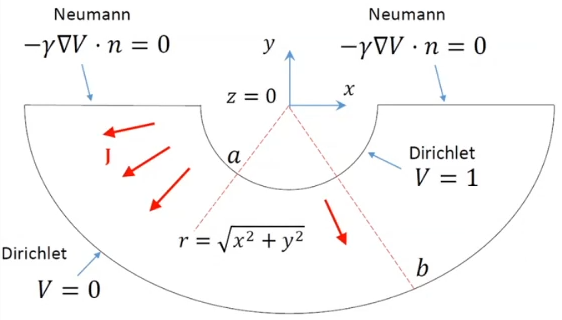
\includegraphics[width=0.5\linewidth]{dispersore_emisferico_FEM}
\end{figure}
Le coordinate utilizzate sono quindi di tipo cilindriche monodimensionali perché anche
nel dominio bidimensionale le grandezze dipendono solo dalla variabile $r$
\begin{align*}
\nabla\cdot (-\gamma\nabla V) &= 0 \\
\frac{1}{r}\frac{d}{dr}\left(-\gamma^*(r)r\frac{dV_{\text{cyl}}}{dr}\right) &= 0
\end{align*}
È possibile utilizzare le coordinate sferiche monodimensionali se si fissa la sezione
$z=0$ in questo modo si trasformano le coordinate sferiche in cartesiane bidimensionali.
Ripetendo i passaggi dell'analisi precedente si ottiene un risultato identico 
a quello della soluzione analitica.

\newpage
\section{Magnetostatica}
Per procedere allo studio della magnetostatica verranno applicate direttamente le 
equazioni di Maxwell alle distribuzioni di sorgenti per determinare i campi.

Legge di Gauss per il campo magnetico, espressa ad una superficie chiusa $\Sigma$ che 
racchiude una regione $\Omega_\Sigma$
$$
\forall\ \Sigma \text{ chiusa di }\mathbb{R}^3\ \oiint_\Sigma \vec{B}\cdot\hat{n}dS = 0
$$
Le linee di $\vec{B}$ sono chiuse al finito o all'infinito oppure
richiudono ergodicamente superfici toroidali. Questa legge afferma che non possono
esistere cariche magnetiche isolate (monopoli magnetici) almeno nell'elettromagnetismo
macroscopico.
In virtù del teorema di Helmholtz i flussi e le circuitazioni vanno assegnati su 
linee chiuse orientate dalla regola della mano destra e superfici da esse racchiuse.
Si ha la legge di Ampère-Maxwell nel caso stazionario 
$$
\forall\ \Gamma \text{ chiusa di } \mathbb{R}^3\ \oint_\Gamma \vec{B}\cdot\hat{t}dl = \mu_0 i_{S_\Gamma}
$$
Le correnti $i_{S_\Gamma}$ sono tutte le correnti ricavabili con il seguente integrale
$$
i_{S_\Gamma} = \iint_{S_\Gamma} \vec{J}\cdot\hat{n}dS
$$

I campi solenoidali in magnetostatica sono $\vec{B}$ e $\vec{J}$ quindi anche
$$
\oiint_\Sigma \vec{J}\cdot\hat{n} dS = 0\ \forall\ \Sigma
$$

I flussi dei campi solenoidali attraverso le superfici dipendono solo dagli orli di
queste ultime e non dalla particolare superficie.
\begin{figure}[H]
\centering
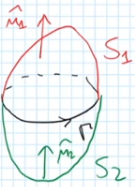
\includegraphics[width = 0.2\linewidth]{flusso_due_superfici}
\end{figure}
Siano $S_1$ e $S_2$ le due superfici la cui unione forma la superficie chiusa $\Sigma$, esse
sono connesse ad un'unica linea $\Gamma$
$$
\oiint_\Gamma \vec{B}\cdot\hat{n}dS = \iint_{S_1} \vec{B}\cdot\hat{n}dS + \iint_{S_2} \vec{B}\cdot\hat{n}dS = 0
$$
con $\hat{n}$ la normale esterna alla superficie chiusa $\Sigma$, sostituendo con le 
rispettive normali orientate si ottiene
$$
\iint_{S_1} \vec{B}\cdot\hat{n}_1dS + \iint_{S_2} \vec{B}\cdot\left(-\hat{n}_2\right)dS = 
\Phi_{S_1} - \Phi_{S_2} = 0 \Rightarrow \Phi_{S_1} = \Phi_{S_2} = \Phi_\Gamma
$$
Si parla quindi di flusso concatenato alla linea $\Gamma$ senza esplicitare l'effettiva
superficie attraverso la quale si sta calcolando il flusso.

\subparagraph{Correnti concatenate}
Si supponga di avere un circuito solido attraversato da corrente come in figura,
si considerano poi due linee $\Gamma_1$ e $\Gamma_2$ che racchiudono il circuito
\begin{figure}[H]
\centering
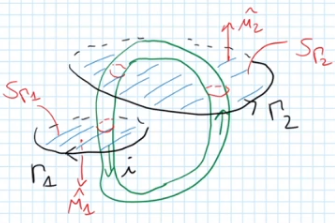
\includegraphics[width = 0.4\linewidth]{circuito_solido_legge_ampere}
\end{figure}

Si definiscono i vettori normali coerentemente alla regola della mano destra
e si riscrive la legge di Ampere-Maxwell per le superfici ottenute
$$
\mu_0 i_{s_\Gamma} =
\begin{cases}
\Gamma_1 : = \mu_0 i\\
\Gamma_2 : = \mu_0(i-i) = 0
\end{cases}
$$

Si potrebbe invece avere un caso con due conduttori che attraversano la stessa superficie
orlata dalla curva $\Gamma$, in questo caso la corrente $i_{S_\Gamma}$ è pari alla
somma delle due correnti che attraversano i conduttori.
\begin{figure}[H]
\centering
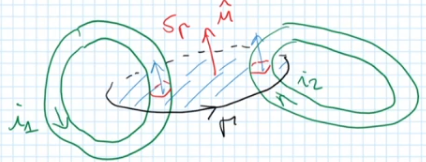
\includegraphics[width = 0.5\linewidth]{due_conduttori_una_superficie}
\end{figure}
\newpage
\paragraph{Distribuzioni di corrente}
Si analizza il caso di una corrente filiforme rettilinea indefinita.
\begin{figure}
\centering
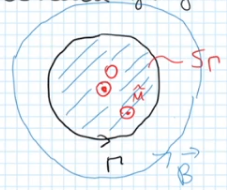
\includegraphics[width=0.3\linewidth]{circuitazione_filiforme}
\end{figure}
$$
\vec{J}(P') = \frac{i}{S}\hat{e}_z
$$
Per simmetria cilindrica della distribuzione di corrente, il campo $\vec{B}$ non può 
dipendere da $z$, data la simmetria di rotazione invece si ha che il campo non dipende 
nemmeno dalla componente azimutale $\varphi$.
$$
\vec{B} = \vec{B}(r) = \cancel{B_r(r)\vec{e}_r} + B_\varphi (r) \vec{e}_\varphi + B_z(r)\vec{e}_z
$$
La componente radiale $B_r(r)\vec{e}_r$ non può esistere perché violerebbe la solenoidalità
di $\vec{B}$.
La componente $\vec{B}_z$ è ammissibile dal punto di vista teorico purché sia costante.

La componente $\vec{B}_\varphi$ si può ricavare con la legge di Ampere-Maxwell
$$
\oint_\Gamma \vec{B}\cdot\hat{t}dl =\mu_0 i_{S_\Gamma} = 2 \pi r B_\varphi(r) = \mu_0 i 
$$
quindi
$$
B_\varphi(r) = \frac{\mu_0}{2 \pi}\frac{i}{r}
$$

\subparagraph{Distribuzione di corrente massiccia}
Sia un conduttore reale di sezione $S$ finita diversa da zero, all'interno del conduttore
si ha un campo 
$$
\vec{J}(P') = \begin{cases}
J_0 \vec{e}_z & r\leq R\\
0 & r > R
\end{cases}
$$
dove $R$ è il raggio del conduttore.
\begin{figure}[H]
\centering
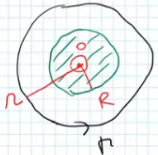
\includegraphics[width = 0.3 \linewidth]{conduttore_massiccio_circuitazione}
\end{figure}
Per le stesse ragioni di simmetria precedenti il campo dipende solo dal raggio $r$ 
ed ha una sola componente tangenziale.
In questo caso però la corrente non è costante se la circuitazione avviene
in una linea interna al conduttore ma dipende dal raggio $r$ della stessa
$$
\oint_\Gamma \vec{B}\cdot\hat{t} dl = \mu_0 \iint_{S_\Gamma}\vec{J}\cdot\hat{n}dS \Leftrightarrow
2\pi r B_\varphi (r) = \begin{cases}
\mu_0 J_0 \pi r^2 & r \leq R \\
\mu_0 J_0 \pi R^2 & r > R
\end{cases}
$$
Semplificando
$$
B_\varphi(r) = \begin{cases}
\frac{\mu_0}{2\cancel{\pi}}\frac{\cancel{\pi}r^{\cancel{2}}}{\cancel{r}}J_0 = \mu_0\frac{J_0}{2}r & r \leq R \\
\frac{\mu_0 J_0 \pi R^2}{2 \pi r} = \frac{\mu_0 i}{2\pi r} & r>R
\end{cases}
$$
All'interfaccia del conduttore non c'è nessuna corrente superficiale, quindi 
la componente del campo è continua attraverso il raggio
$$
B_\varphi(R^-) = B_\varphi(R^+)
$$
Il campo cresce linearmente per $0 < r \leq R$ e poi decresce come $\frac{1}{r}$.

\subparagraph{Distribuzione di corrente piana indefinita}
Si immagina un parallelepipedo non limitato attraversato da una certa corrente,
di spessore $\Delta$. Si colloca l'origine del sistema di riferimento in un punto 
del suo piano di mezzeria. 
\begin{figure}[H]
\centering
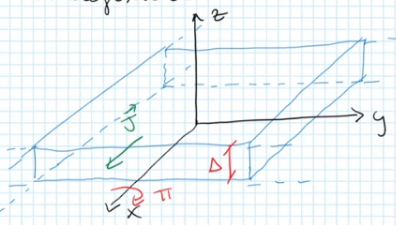
\includegraphics[width = 0.4\linewidth]{lastra_piana_magnetostatica}
\end{figure}
Si ha una distribuzione uniforme lungo la coordinata $x$, $\vec{J} = J_0 \vec{e}_x $ quando
$|z| \leq \frac{\Delta}{2}$, invariante per traslazione nel piano $(x,y)$ quindi
$$
\vec{B} = \vec{B}(z) = B_x(z)\vec{e}_x + B_y(z)\vec{e}_y + B_z(z)\vec{e}_z
$$

Si suppone di ruotare il piano di $\pi$ attorno l'asse $x$, tutte le componenti cambiano
segno eccetto $B_x$ che ha quindi simmetria pari:
\begin{align*}
&B_x(z) = B_x(-z) \text{ funzione pari}\\
&B_y(z) = -B_y(-z) \text{ funzione dispari} \\
&B_z(z) = -B_z(-z) \text{ funzione dispari}
\end{align*}

Si considera ora una sezione del piano ed una linea rettangolare $\Gamma$ di orientamento
antiorario
di coordinate $(x_1,x_2) \text{ e } (z_1,z_2)$ al di sopra della distribuzione piana.
La corrente concatenata è pari a zero, si svolge comunque l'integrale di linea.
\begin{figure}[H]
\centering
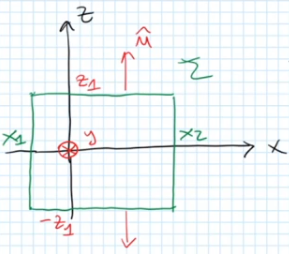
\includegraphics[width = 0.3\linewidth]{integrale_attraverso_lastra_conduttrice_magnetostatica}
\end{figure}
$$
\oint_\Gamma \vec{B}\cdot\hat{t}dl = 0 = \int_{x_1}^{x_2} B_x (z_1)dx + \cancel{\int_{z_1}^{z^2}B_z(x_2)dz} + \int_{x_2}^{x_1} B_x (z_2)dx + \cancel{\int_{z_2}^{z^1}B_z(x_1)dz} 
$$
Sfruttando la simmetria dispari della componente lungo $z$ si annullano i due termini in 
$dz$.
Quindi
$$
(x_2-x_1)\left[B_x(z_1) - B_x(z_2)\right] = 0 \ \forall \ x_1,x_2
$$
ma per la legge di annullamento del prodotto se $x_1\neq x_2$
$$
B_x(z_1) = B_x(z_2)\ \forall\ z_1,z_2 > h \Rightarrow B_x(z) = \text{cost} = B_{x_0},\ |z| > h
$$

Per analizzare la solenoidalità di $\vec{B}$ si considera ora un parallelepipedo
simmetrico rispetto al piano $(x,y)$.
$$
\oiint_\Sigma \vec{B}\cdot\hat{n}dS = 0 = \int_{x_1}^{x_2}dx \int_{y_1}^{y_2} dy B_z(z_1)
- \int_{x_1}^{x_2}dx \int_{y_1}^{y_2} dy B_z(-z_1) + \cancel{\int_{x_1}^{x_2}dx \int_{-z_1}^{z_1} dz B_y(z)} -
$$
$$
- \cancel{\int_{x_1}^{x_2}dx\int_{-z_1}^{z_1}dzB_y(z)} + \cancel{\int_{y_1}^{y_2}dy\int_{-z_1}^{z_1} dzB_x} - \cancel{\int_{y_1}^{y_2}dy\int_{-z_1}^{z_1}dzB_x} = 0
$$

Gli ultimi due termini si elidono perché $B_x$ è costante come visto precedentemente,
il terzo e il quarto invece sono identici ma di segno opposto.

In conclusione si vede che gli integrali delle facce parallele al piano $(x,y)$ hanno
differenza nulla
$$
(x_1-x_2)(y_1-y_2)[B_z(z_1)-B_z(z_2)] = (x_1-x_2)(y_1-y_2)[2B_z(z_1)] = 0 \Rightarrow B_z(z_1) = 0\ \forall z_1
$$

Per analizzare la $B_y$ si considera il piano $(y,z)$ e una linea ancora orientata in verso 
antiorario
\begin{figure}[H]
\centering
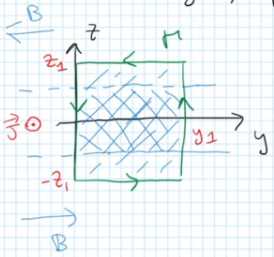
\includegraphics[width = 0.3\linewidth]{integrale_attraverso_lastra_conduttrice_magnetostatica_2}
\end{figure}
$$
\oint_\Gamma\vec{B}\cdot\hat{t}dl =\mu_0 2h\cancel{y_1}J_0 = \cancel{y_1}B_y(-z_1) - \cancel{y_1}B_y(z_1)
$$
$$
\mu_0 \cancel{2} h J_0 = -\cancel{2}B_y(z_1)
$$
Quindi si ottiene la componente del campo che concatena ancora una volta la corrente
$$
B_y(z_1) = -\mu_0 J_0 h
$$

Se si definisce la corrente superficiale $J_0 h = \frac{J_s}{2}$ si può affermare che
$$
B_y(z) = \begin{cases}
-\mu_0\frac{J_s}{2} & z > h\\
\mu_0\frac{J_s}{2} & z < -h
\end{cases}
$$
Passando al limite per $h \to 0^+$ si ottiene il campo prodotto da una distribuzione
superficiale di corrente e che 
$$
\hat{n}\times(\vec{B}_2-\vec{B}_1) = \mu_0 \vec{J_s}
$$
\begin{figure}[H]
\centering
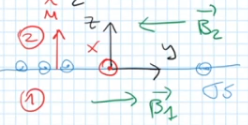
\includegraphics[width=0.4\linewidth]{campo_magnetico_lastra_piana}
\end{figure}
